\section{Evaluation Data} \label{sec:body_evaluation_data}

As I will not conduct a user study my approach of for evaluating various features will be to analyze the difference of the metric scores between distinct groups of mnemonics. I have in total gathered data from 4 groups. High quality examples of mnemonics have been randomly sampled from  \emph{wanikani.com}. The website's popularity in the field of Japanese Kanji learning should be evidence enough to indicate decent effectiveness.

As I was not able to find examples for the low end, I instead opted to generated them with the only requirement that the input words are found in the output. I chose a GPT-2 model for this task.

Additionally, two more example groups have been generated using GPT-3 with different prompts, one asking the model to come up with a paragraph that must include input words and another that prompted it to output a mnemonic story based on the input words.

A total of 760 mnemonics with a group specific sample size of 190 have been collected for evaluation. Following an example of each group is shown given the input words \emph{plow, drunkard and planting}. They are derived from the Kanji 栽 which means \emph{planting}.
\begin{description}
    \item[WaniKani] A \emph{drunkard} gets his hands on a \emph{plow} and starts \emph{planting} right away. Drunk people are surprisingly good at \emph{planting}, especially when they have machines to help them do it. Picture a drunk guy laughing and plowing a field and \emph{planting} seeds. He wouldn't do this if he was sober, but drunk people can't help themselves.
    \item[GPT-2]  This is a \emph{plow} \emph{drunkard}'s guide to \emph{planting} trees in your yard. If you don't know what I'm talking about, check out my previous post on the subject: How To Plant A Tree In Your Backyard (And Why You Should Do It). This time we'll be looking at different types of tree species and how they can
    \item[GPT-3 paragraph] The \emph{drunkard} stumbled out of the bar and made his way to the nearby farm, where he began to \emph{plow} the fields for the upcoming planting season. He worked tirelessly for hours, his mind foggy with alcohol, until the fields were ready for the \emph{planting}.
    \item[GPT-3 mnemonic] Once upon a time, there was a \emph{drunkard} who stumbled into a field with a \emph{plow} in hand. He decided to \emph{plant} some seeds he had found in his pocket, and with a few clumsy swipes of the plow, he was able to make some furrows in the field. With a satisfied smile, he watched as the seeds he \emph{planted} took root. 
\end{description}
For the GPT-3 prompts I used the \texttt{text-davinci-003} GPT-3 model which is the most powerful of its evolution at the time of this writing. The used prompts are listed below.
\begin{description}
    \item[Paragraph] Write a short paragraph that includes the following words: drunkard, plow, planting
    \item[Mnemonic] Write a short paragraph long mnemonic story that is based on and must include the words: drunkard, plow, planting
\end{description}
For the low end examples I used a 1.5B parameter version of GPT-2 \cite{radford2019language}. Since a non fine-tuned GPT-2 model is not very good in providing sensible output given similar prompts to the ones above, I had to use \emph{constrained beam search} in order to ensure the requirement of including all input words.

Instead of just using the most likely token at each generation step given the previous tokens, commonly referred to as \emph{greedy search}, beam search keeps track of the $n$ most probable candidates at every time step and uses them as context for the next iteration \cite{kim2022guiding}. The constrained version of the method forces the tokens that must be included in the output as possible extensions of the previous tokens and divides candidates into so-called \emph{banks}. Each bank is defined by how many of the constrained tokens are included in the candidate. Following, the $n$ candidates for the next iteration are selected by round-robin, taking the most likely candidate from each bank until $n$ is reached. The banks are also sorted by how many of the constraint tokens they include in their candidates. The process is visualized in Figure \ref{figure:constrained_beam_search_example}.  
\begin{figure}
    \centering
    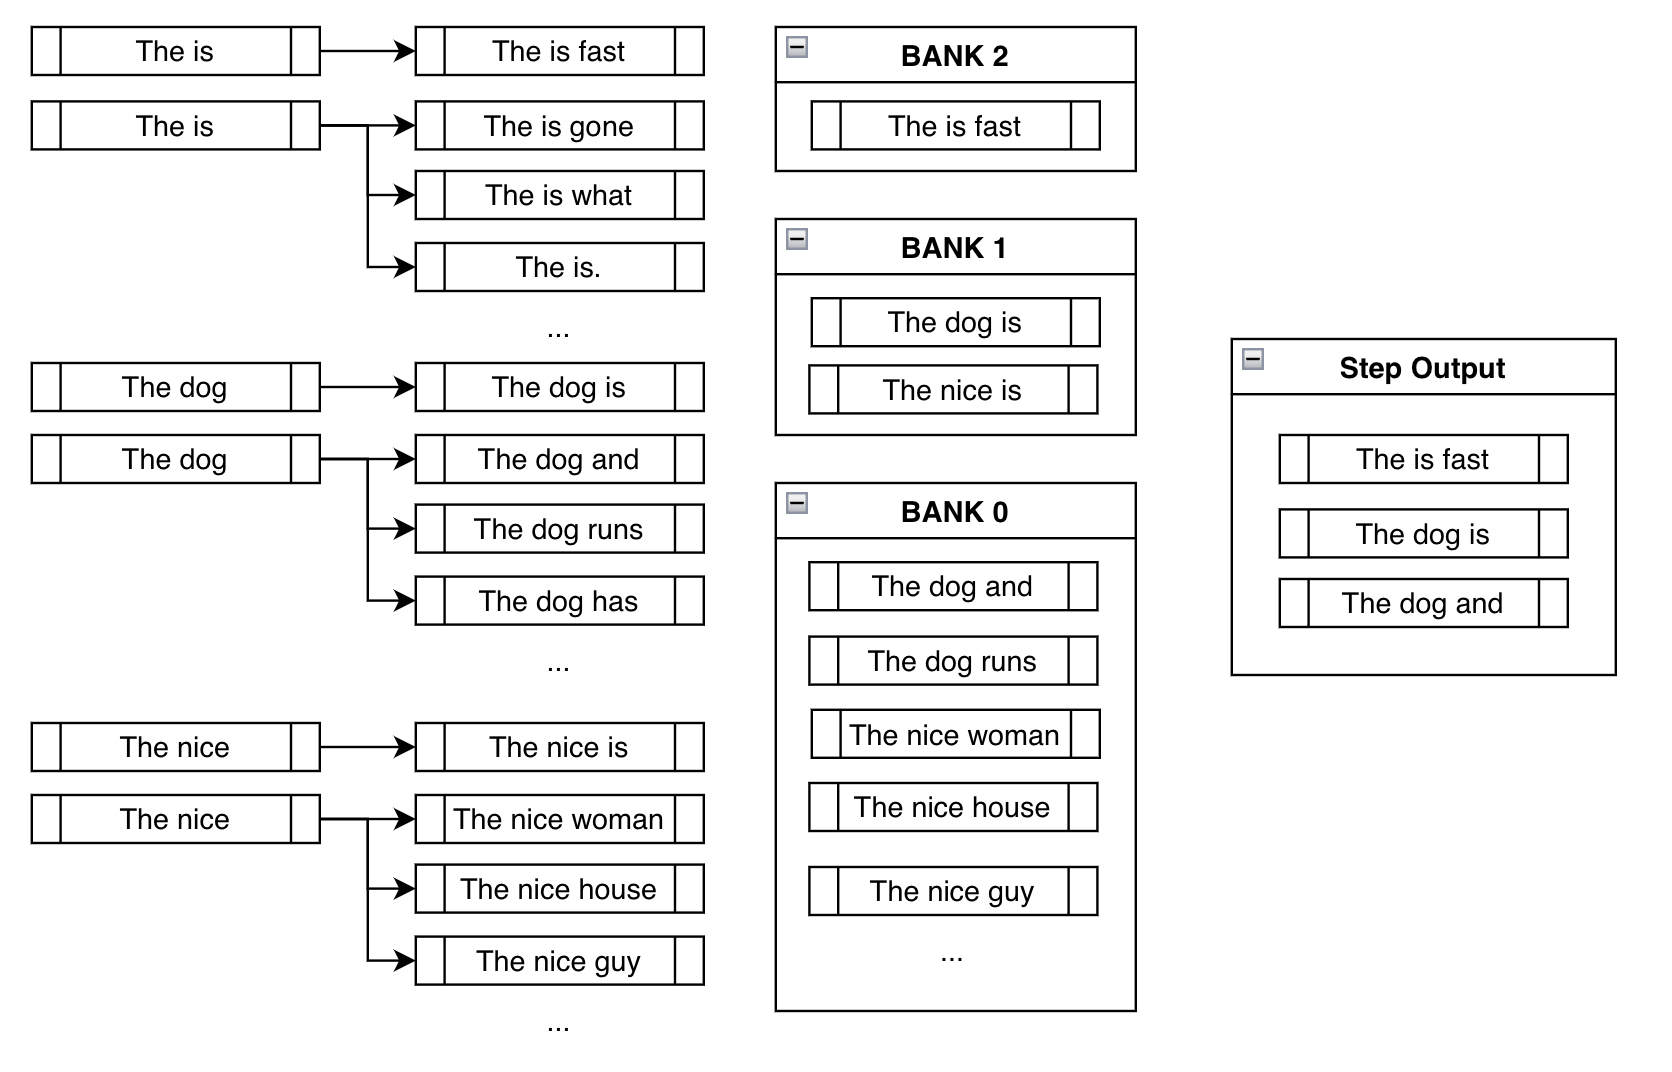
\includegraphics[width=400pt]{resources/cbeam_2.jpg}
    \caption{Constrained beam search example with forcing the phrase "is fast" \cite{kim2022guiding}}
    \label{figure:constrained_beam_search_example}
\end{figure}